\section{Lines}

In the Euclidean plane, a line is typically defined by the equation:
\[aX+bY+c=0\]
However, in the homogeneous plane, lines are represented as:
\[a\dfrac{x}{w}+b \dfrac{y}{w}+c=0 \Longrightarrow ax+by+cw=0\]
This equation can also be expressed using two vectors, denoted as $l^T$ and $x$, as follows:
\[\begin{bmatrix} a & b & c \end{bmatrix} \begin{bmatrix} x \\ y \\ w \end{bmatrix}=0\]
Here, the vector $l={\begin{bmatrix} a & b & c \end{bmatrix}}^T$, and all its nonzero multiples represent a line.  
This representation adheres to the homogeneity property: any vector $l$ is equivalent to all its nonzero multiples, denoted as $\lambda l$, where $\lambda\neq 0$, since they denote the same line. 
The coefficients $a$, $b$, and $c$ are referred to as the homogeneous parameters of the line.

Similar to numbers, there exist numerous equivalent representations for a single line, specifically all nonzero multiples of the unit normal vector. 
The null vector, however, does not represent any lines.
\begin{definition}
    The \emph{projective dual plane} is defined as: 
    \[\mathbb{P}^2=\{{\begin{bmatrix} a & b & c \end{bmatrix}}^T \in \mathbb{R}^3\}-\{{\begin{bmatrix} 0 & 0 & 0 \end{bmatrix}}^T\}\]
\end{definition}

\begin{property}
    If the third parameter is zero, denoted as ${l=\begin{bmatrix} a & b & 0 \end{bmatrix}}^T$, then the line passes through the point $\begin{bmatrix} 0 & 0 \end{bmatrix}$. 
\end{property}
\begin{property}
    In the Euclidean plane, the direction $\begin{bmatrix} a & b \end{bmatrix}$ is perpendicular to the line represented by ${l=\begin{bmatrix} a & b & c \end{bmatrix}}^T$.
\end{property}
\begin{property}
    Two lines, ${l=\begin{bmatrix} a & b & c \end{bmatrix}}^T$ and ${l=\begin{bmatrix} a & b & c^{'} \end{bmatrix}}^T$, are considered parallel when they share the same direction, which is represented by $[b,-a]$.
\end{property}
\begin{example}
    The Cartesian axes are defined as: 
    \[l_x={\begin{bmatrix} 0 & 1 & 0 \end{bmatrix}}^T\]
    \[l_y={\begin{bmatrix} 1 & 0 & 0 \end{bmatrix}}^T\]
\end{example}
In this context, the incidence relation of a line $l^Tx=0$ is defined when the point $x$ lies on the line $l$ or when the line $l$ goes through the point $x$. 
\begin{definition}
    The line 
    \[\begin{bmatrix} 0 & 0 & 1 \end{bmatrix} \begin{bmatrix} x \\ y \\ w \end{bmatrix}=w=0\] 
    is called the \emph{line at the infinity}, denoted as $l_{\infty}={\begin{bmatrix} 0 & 0 & 1 \end{bmatrix}}^T$. 
\end{definition}
The principle of duality between points and lines states that the incidence relation is commutative since the dot product is commutative.

To find the intersection of two lines $l_1$ and $l_2$, the following condition is imposed:
\[\begin{bmatrix} l_1^T \\ l_2^T \end{bmatrix} x = \begin{bmatrix} 0 \\ 0 \end{bmatrix}\]
This equation leads to finding the right null space of the first column vector:
\[x=\textnormal{RNS}\left(\begin{bmatrix}l_1^T \\ l_2^T \end{bmatrix} \right)\]
The system is under-determined, meaning there is only one intersection point between two lines, which can be represented in multiple ways in homogeneous coordinates.
In 2D projective geometry, the vector $x$ is orthogonal to both lines and can be found using the cross product:
\[x=l_1 \times l_2\]
\begin{example}
    Suppose we have two parallel lines, $l_1={\begin{bmatrix} a & b & c_1 \end{bmatrix}}^T$ and $l_2={\begin{bmatrix} a & b & c_2 \end{bmatrix}}^T$. 
    The point that is common to both lines can be found using the system:
    \[
        \begin{cases}
            ax+by+c_1w=0 \\
            ax+by+c_2w=0
        \end{cases}
    \]
    The solution is ${x=\begin{bmatrix} b & -a & 0 \end{bmatrix}}^T$, which represents the point at infinity along the direction of both lines.
\end{example}

The line passing through two points can be determined using the dual of the previous problem, expressed as:
\[\begin{bmatrix} x_1^T \\ x_2^T \end{bmatrix} l = \begin{bmatrix} 0 \\ 0 \end{bmatrix}\]
In 2D, this simplifies to: 
\[l=x_1 \times x_2\] 
\begin{property}
    A point $x$ obtained by a linear combination $x=\alpha x_1+\beta x_2$ of two points $x_1$ and $x_2$ lies on the line $l$ through $x_1$ and $x_2$. 
\end{property}
\begin{proof}
    The line $l$ passing through both points satisfies  $l^Tx_1=0$ and  $l^Tx_2=0$. 
    By adding $\alpha$ times the first equation to $\beta$ times the second one, we obtain: 
    \[0=l^T\left( \alpha x_1+\beta x_2 \right)=l^Tx=0\]
\end{proof}
This establishes the duality between co-linear and concurrent.
\begin{theorem}
    For any true sentence containing the words: point, line, is on, goes through, co-linear and concurrent there exists a dual sentence (also true) obtained by replacing each occurrence of:
    \begin{itemize}
        \item Point $\Leftrightarrow$ line. 
        \item Is on $\Leftrightarrow$ goes through.
        \item Co-linear $\Leftrightarrow$ concurrent. 
    \end{itemize}
\end{theorem}
Within the euclidean plane, the direction normal to the line $l={\begin{bmatrix} a & b & c \end{bmatrix}}^T$ is represented by $\begin{bmatrix} a & b \end{bmatrix}$. 
This relationship between lines can be explained by understanding that the angle between two lines is equal to the angle between their respective normal vectors. 
The formula for the angle between two vectors is:
\[\cos\theta=\dfrac{u \cdot v}{\left\lvert u \right\rvert \left\lvert v \right\rvert}\] 
This applies to the angle between two lines $l_1={\begin{bmatrix} a_1 & b_1 & c_1 \end{bmatrix}}^T$ and $l_2={\begin{bmatrix} a_2 & b_2 & c_2 \end{bmatrix}}^T$. 
In this context, it is the angle between their respective normal directions $\begin{bmatrix} a_1 & b_1 \end{bmatrix}$ and $\begin{bmatrix} a_2 & b_2 \end{bmatrix}$, which can be calculated as follows:
\[\cos\theta=\dfrac{a_1a_2+b_1b_2}{\sqrt{\left( a_1^2 + b_1^2 \right)\left( a_2^2 + b_2^2 \right)}}\]

Now, consider a line with four points related as follows:
\[X_1=\alpha_1Y+\beta_1Z\]
\[X_2=\alpha_2Y+\beta_2Z\]
The cross ratio is given by:
\[CR_{X_1,X_2,Y,Z}=\dfrac{c-a}{c-b}/\dfrac{d-a}{d-b}=\dfrac{\beta_1/\alpha_1}{\beta_2/\alpha_2}\]
\begin{figure}[H]
    \centering
    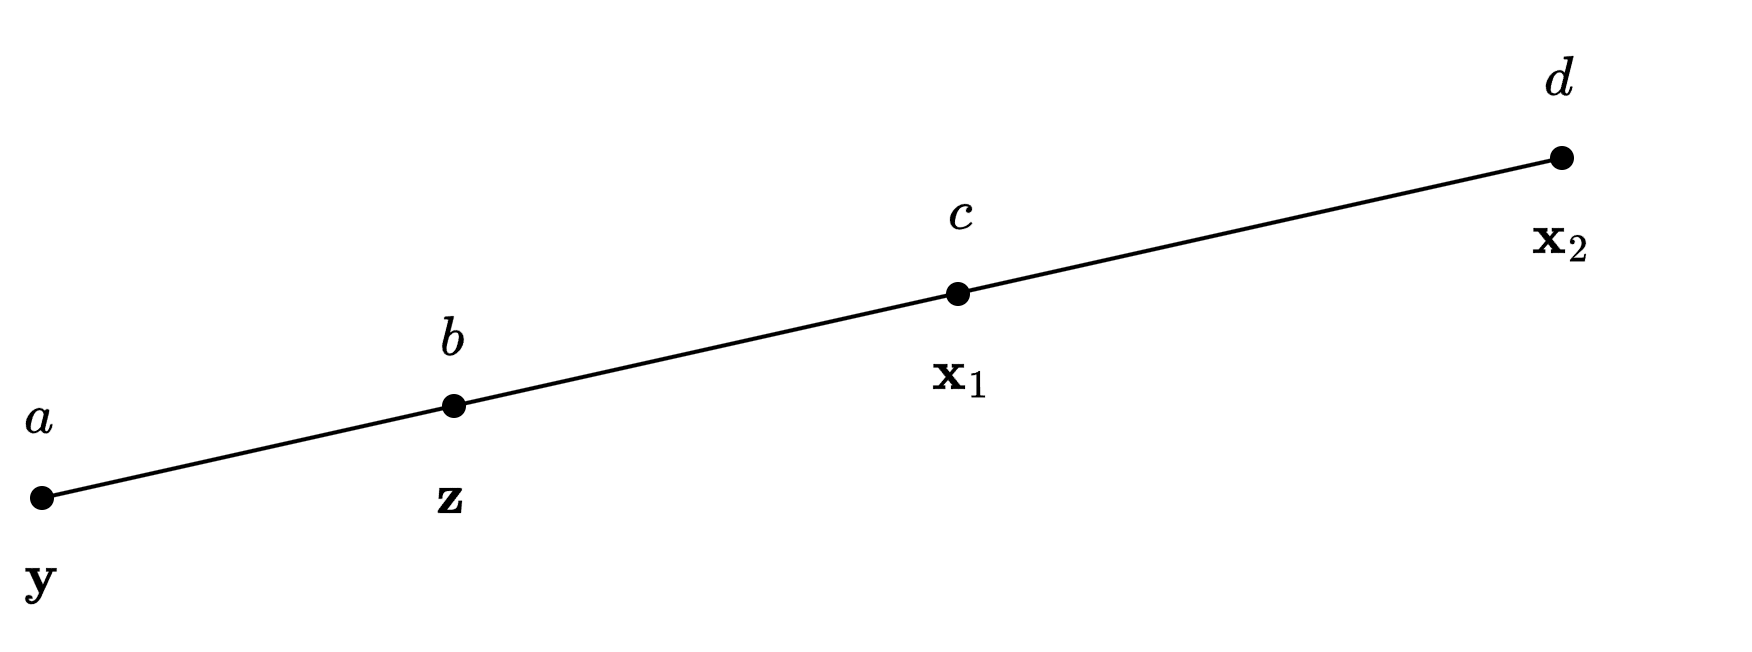
\includegraphics[width=0.25\linewidth]{images/line.png}
    \caption{Line with the point of previous problem}
\end{figure}
\begin{proof}
    Since the abscissae are proportional, the abscissae can be replaced by the $X$ coordinate, as illustrated in the figure below:
    \begin{figure}[H]
        \centering
        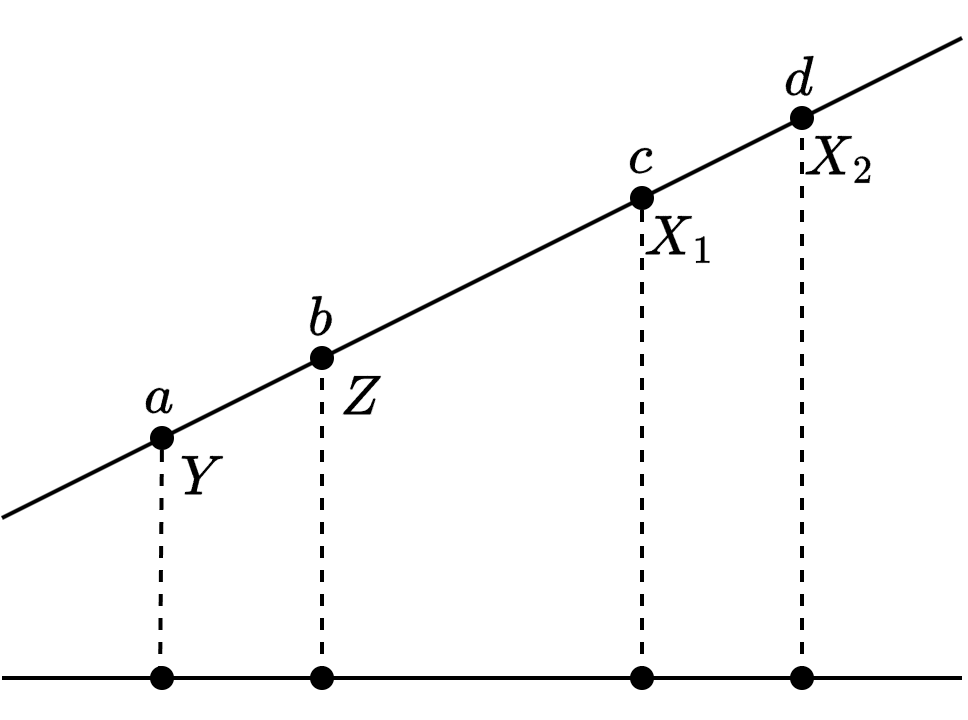
\includegraphics[width=0.3\linewidth]{images/abscissae.png}
    \end{figure}
    The relation:
    \[CR_{X_1,X_2,Y,Z}=\dfrac{c-a}{c-b}/\dfrac{d-a}{d-b}\]
    still holds. 
    If we consider $Y={\begin{bmatrix} y & * & v \end{bmatrix}}^T$ and $Z={\begin{bmatrix} z & * & w \end{bmatrix}}^T$, we can determine that:
    \[ X_1=\begin{bmatrix} \alpha_1y+\beta_1z \\ * \\ \alpha_1v+\beta_1w \end{bmatrix} \:\:\:\:\:\:\:\:\:\:\:\: X_2=\begin{bmatrix} \alpha_2y+\beta_2z \\ * \\ \alpha_2v+\beta_2w \end{bmatrix}\]
    The difference between the $X$ coordinates of $X_1$ and $Y$ is calculated as:
    \[c-a=\dfrac{\beta_1(zv-yw)}{(\alpha_1y+\beta_1z)v}\]
    Similarly, the difference between the $X$ coordinates of $X_1$ and $Z$ is:
    \[c-b=\dfrac{-\alpha_1(zv-yw)}{(\alpha_1y+\beta_1z)w}\]
    By substituting these expressions, we obtain:
    \[ \dfrac{c-a}{c-b}=-\dfrac{\beta_1w}{\alpha_1v} \:\:\:\:\:\:\:\:\:\:\:\: \dfrac{d-a}{d-b}=-\dfrac{\beta_2w}{\alpha_2v}\]
\end{proof}